% This is a Basic Assignment Paper but with like Code and stuff allowed in it, there is also url, hyperlinks from contents included. 

\documentclass[11pt]{article}

% Preamble

\usepackage[margin=1in]{geometry}
\usepackage{amsfonts, amsmath, amssymb}
\usepackage{fancyhdr, float, graphicx}
\usepackage[utf8]{inputenc} % Required for inputting international characters
\usepackage[T1]{fontenc} % Output font encoding for international characters
\usepackage{fouriernc} % Use the New Century Schoolbook font
\usepackage[nottoc, notlot, notlof]{tocbibind}
\usepackage{listings}
\usepackage{xcolor}
\usepackage{blindtext}
\usepackage{hyperref}
\hypersetup{
    colorlinks=true,
    linkcolor=black,
    filecolor=magenta,      
    urlcolor=cyan,
    pdfpagemode=FullScreen,
    }

\definecolor{codegreen}{rgb}{0,0.6,0}
\definecolor{codegray}{rgb}{0.5,0.5,0.5}
\definecolor{codepurple}{rgb}{0.58,0,0.82}
\definecolor{backcolour}{rgb}{0.95,0.95,0.92}

\lstdefinestyle{mystyle}{
    backgroundcolor=\color{backcolour},   
    commentstyle=\color{codegreen},
    keywordstyle=\color{magenta},
    numberstyle=\tiny\color{codegray},
    stringstyle=\color{codepurple},
    basicstyle=\ttfamily\footnotesize,
    breakatwhitespace=false,         
    breaklines=true,                 
    captionpos=b,                    
    keepspaces=true,                 
    numbers=left,                    
    numbersep=5pt,                  
    showspaces=false,                
    showstringspaces=false,
    showtabs=false,                  
    tabsize=2
}

\lstset{style=mystyle}

% Header and Footer
\pagestyle{fancy}
\fancyhead{}
\fancyfoot{}
\fancyhead[L]{\textit{\Large{Information and Cycbersecurity - 2nd Year B. Tech}}}
%\fancyhead[R]{\textit{something}}
\fancyfoot[C]{\thepage}
\renewcommand{\footrulewidth}{1pt}



% Other Doc Editing
% \parindent 0ex
%\renewcommand{\baselinestretch}{1.5}

\begin{document}

\begin{titlepage}
	\centering

	%---------------------------NAMES-------------------------------

	\huge\textsc{
		MIT World Peace University
	}\\

	\vspace{0.75\baselineskip} % space after Uni Name

	\LARGE{
		Information and Cybersecurity\\
		Second Year B. Tech, Semester 1
	}

	\vfill % space after Sub Name

	%--------------------------TITLE-------------------------------

	\rule{\textwidth}{1.6pt}\vspace*{-\baselineskip}\vspace*{2pt}
	\rule{\textwidth}{0.6pt}
	\vspace{0.75\baselineskip} % Whitespace above the title



	\huge{\textsc{
			Classical Cryptographic Technique Implementations\\
			\textit{"Simplified Advaned Encryption Standard"}
		}} \\



	\vspace{0.5\baselineskip} % Whitespace below the title
	\rule{\textwidth}{0.6pt}\vspace*{-\baselineskip}\vspace*{2.8pt}
	\rule{\textwidth}{1.6pt}

	\vspace{1\baselineskip} % Whitespace after the title block

	%--------------------------SUBTITLE --------------------------	

	\LARGE\textsc{
		Lab Assignment 3
	} % Subtitle or further description
	\vfill

	%--------------------------AUTHOR-------------------------------

	Prepared By
	\vspace{0.5\baselineskip} % Whitespace before the editors

	\Large{
		Krishnaraj Thadesar \\
		Cyber Security and Forensics\\
		Batch A1, PA 20
	}


	\vspace{0.5\baselineskip} % Whitespace below the editor list
	\today

\end{titlepage}


\tableofcontents
\thispagestyle{empty}
\clearpage

\setcounter{page}{1}

\section{Aim}
Write a program using JAVA or Python or C++ to implement S-AES symmetric key
algorithm.

\section{Objectives}
To understand the concepts of block cipher and symmetric key cryptographic
system.

\section{Theory}

\subsection{What is Simplified AES?}
S-AES is to AES as S-DES is to DES. In fact, the structure of S-AES is exactly the
same as AES. The differences are in the key size (16 bits), the block size (16 bits) and the number
of rounds (2 rounds).

The Advanced Encryption Standard (AES) is a widely-used symmetric-key encryption algorithm that is used to encrypt and decrypt data. The simplified AES algorithm is a simplified version of the AES algorithm that is often used as a teaching tool to help people understand how AES works.

The simplified AES algorithm operates on a 4x4 matrix of bytes called a "state." The algorithm consists of several rounds, each of which performs a series of operations on the state. The number of rounds depends on the key size: 10 rounds for a 128-bit key, 12 rounds for a 192-bit key, and 14 rounds for a 256-bit key.

The simplified AES algorithm is a simplified version of the AES algorithm that is often used as a teaching tool to help people understand how AES works.


\begin{figure}[H]
	\centering
	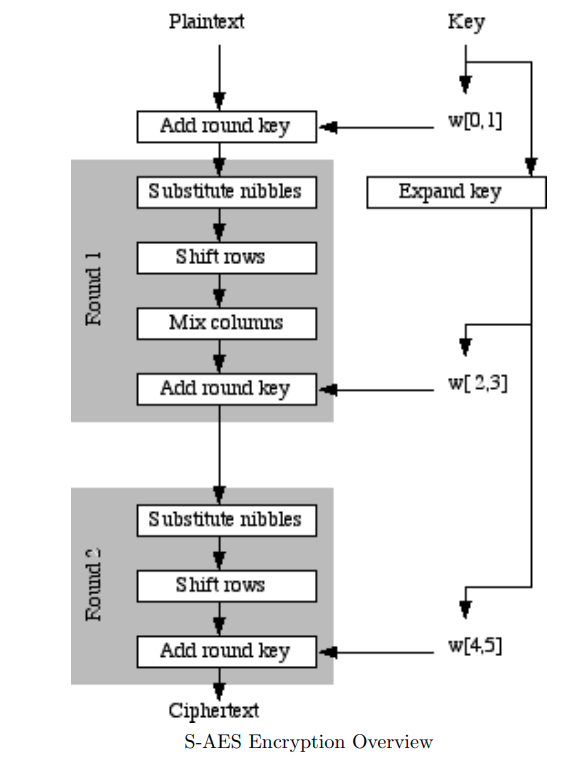
\includegraphics[scale=0.5]{saes.png}
	\caption{}
\end{figure}

\subsection{Key Expansion}
The key expansion function is the same as AES. The key is expanded to 32 bits and
then split into two 16-bit keys. The first key is used in the first round and the second key is used in the second round. 
\subsection{Constants}

\subsection{Substitution}
In this step, each byte in the state is replaced by another byte using a substitution table called the S-box. The S-box is a fixed table that maps each possible byte value to another byte value. The byte value is used to look up a corresponding value in the S-box. The substitution is done in a byte-wise manner.
\subsection{Shift Rows}

% \subsection{Mix Columns}

% \subsection{Key Expansion Function (g())}

% \subsection{Round Function}

% \subsection{Encryption}

% \subsection{Decryption}

Here are the steps of one round of the simplified AES algorithm:

\begin{enumerate}
	\item SubBytes: In this step, each byte in the state is replaced by another byte using a substitution table called the S-box.
	
	\item ShiftRows: In this step, the bytes in each row of the state are shifted to the left. The first row is not shifted, the second row is shifted by one byte to the left, the third row is shifted by two bytes to the left, and the fourth row is shifted by three bytes to the left.
	
	\item MixColumns: In this step, each column of the state is multiplied by a fixed matrix. This is a bit more complex than the other steps, but it essentially "mixes" the bytes in each column.
	
	\item AddRoundKey: In this step, each byte in the state is XORed with a byte from the key schedule. The key schedule is derived from the original key using a key expansion algorithm.
\end{enumerate}
	
\section{Platform}
\textbf{Operating System}: Arch Linux x86-64 \\
\textbf{IDEs or Text Editors Used}: Visual Studio Code\\
\textbf{Compilers or Interpreters} : Python 3.10.1\\

\section{Input and Output}
\begin{verbatim}
    Enter Text to be encrypted via S-AES:AES is much better than DES
    Enter 4 digit Key to be used for encryption:9087
    Your Cipher Text is:  
                          HéWõëd¸½Kùд^#EGã'
    The decrypted plain text is:  AES is much better than DES
\end{verbatim}
\section{Code}
\lstinputlisting[language=Python, caption="Fiestal Cipher"]{../Programs/Assignment_3/Simplified_AES.py}

\section{Conclusion}
Thus, learnt about the different kinds of ciphers, classical cryptographic techniques, and how to implement some of them in python.
\clearpage

\section{FAQ}

\begin{enumerate}
	\item \textbf{Differentiate between DES and AES.}\\
	      \textbf{AES: }
	      \begin{enumerate}
		      \item AES stands for advanced encryption standard.
		      \item The key length can be 128 bits, 192 bits, or 256 bits.
		      \item The rounds of operations per key length are as follows: 128 bits: 10 192 bits: 12 256 bits: 14
		      \item AES is based on a substitution and permutation network.
		      \item AES is considered the standard encryption algorithm in the world and is more secure than DES.
		      \item Key Addition, Mix Column, Byte Substitution, and Shift Row.
		      \item AES can encrypt plaintext of 128 bits.
		      \item AES was derived from the Square Cipher.
		      \item AES was designed by Vincent Rijmen and Joan Daemen.
		      \item There are no known attacks for AES.
	      \end{enumerate}

	      \textbf{DES: }
	      \begin{enumerate}
		      \item DES stands for data encryption standard.
		      \item The key length is 56 bits.
		      \item There are 16 identical rounds of operations.
		      \item DES is based on the Feistel network.
		      \item DES is considered to be a weak encryption algorithm; triple DES is a more secure encryption algorithm.
		      \item Substitution, XOR Operation, Permutation, and Expansion.
		      \item DES can encrypt plaintext of 64 bits.
		      \item DES was derived from the Lucifer Cipher.
		      \item DES was designed by IBM.
		      \item Brute force attacks, differential cryptanalysis, and linear cryptanalysis.
	      \end{enumerate}

	\item \textbf{What are the different advantages and Limitations of AES?}\\
	      \textbf{Advantages: }\\
	      \begin{enumerate}
		      \item Following are the benefits or advantages of AES:
		      \item As it is implemented in both hardware and software, it is most robust security protocol.
		      \item It uses higher length key sizes such as 128, 192 and 256 bits for encryption. Hence it makes AES algorithm more robust against hacking.
		      \item It is most common security protocol used for wide various of applications such as wireless communication, financial transactions, e-business, encrypted data storage etc.
		      \item It is one of the most spread commercial and open source solutions used all over the world.
		      \item No one can hack your personal information.
		      \item For 128 bit, about 2128 attempts are needed to break. This makes it very difficult to hack it as a result it is very safe protocol.
	      \end{enumerate}


	      \textbf{Limitations: }\\
	      \begin{enumerate}
		      \item It uses too simple algebraic structure.
		      \item Every block is always encrypted in the same way.
		      \item Hard to implement with software.
		      \item AES in counter mode is complex to implement in software taking both performance and security into considerations.
	      \end{enumerate}

\end{enumerate}


\end{document}